\documentclass[10pt]{article}

%defines page size and margins
\usepackage{geometry}
\geometry{
    letterpaper,
    left=1in,
    right=1in,
    top=1in,
    bottom=1in,
}

%Sets spacing for entire document
\usepackage{setspace}
\singlespacing

%Package for reducing space in between list items
\usepackage{enumitem}

%urls
\usepackage{hyperref}

%multirow for tables
\usepackage{multirow}

%Math symbols
\usepackage{gensymb}
\usepackage{siunitx}

%numberless captions
\usepackage{caption}

%Image path
\usepackage{graphicx}
\graphicspath{ {/} }

%Used for adjusting images
\usepackage[export]{adjustbox}

%For floating images
\usepackage{float}

\begin{document}
\title{Laboratory Five --- Transient Response}
\date{November 17, 2017}
\author{Rishabh Shah\\ 4655 4192\\ \\ Partner: Matthew Remillard}
\maketitle
\newpage

\section*{Pre-Lab}
\subsection*{I}
\subsubsection*{a}
$\tau = RC = 1k\Omega \cdot 0.1 \times 10^{-6} = 1 \times 10^{-4} s$

\subsubsection*{b}
$v_0 = 1V$\\
$v_R(t) = 1 -v_c(t)$\\
$v_c(t) = v_0(1-e^{\frac{-t}{\tau}} = 1-e^{\frac{0.001}{0.0001}} = 1V$\\
\begin{table}[H]
	\centering
	\begin{tabular}{ll}
		\hline
		Element & $v_{PPK} (V)$\\
		\hline
		$v_{C,PPK}$ & 1\\
		$v_{R,PPK}$ & 1\\
		\hline
	\end{tabular}
	\caption{Data for Pre-Lab 1b}
\end{table}

\subsubsection*{c}
\noindent We can assume the circuit reaches steady state because there are more than five time constants in that time period.

\subsubsection*{d}
\noindent The capacitor must charge, so $v_c$ increases with time. As this occurs, the voltage across the resistor must drop, as $v_0 = v_R + v_c$.

\subsection*{II}
\subsubsection*{a}
\noindent $v_c$ charges when $v_0 = 1V$ and discharges when $v_0 = 0V$. Since $v_0 = v_R + v_c$, $v_R$ is 1 when $v_c$ is 0 and $v_R$ is 0 when $v_c$ is 1.

\subsubsection*{b}
$v_c(t) = 1-e^{\frac{0.001}{0.0001}} = 1V$\\
$v_0 = v_R + v_c$
\begin{table}[H]
	\centering
	\begin{tabular}{ll}
		\hline
		Element & $v_{PPK} (V)$\\
		\hline
		$v_{C,PPK}$ & 1\\
		$v_{R,PPK}$ & 2\\
		\hline
	\end{tabular}
	\caption{Data for Pre-Lab 2b}
\end{table}

\subsection*{III}
\subsubsection*{a}
$v_c(t) = 1-e^{\frac{-2.5\times10^{-4}}{0.0001}} = 0.918V$\\
\noindent The time constant has increased by a factor of 2.5, which means the circuit has not reached steady state.

\subsubsection*{b}
$f_{max} = 1000Hz$\\
\noindent The circuit has not reached steady state because five time constants have not passed.

\subsection*{IV}
\subsubsection*{a}
$\omega_0 = 422.577$\\

\subsubsection*{b}
\begin{table}[H]
	\centering
	\begin{tabular}{lllll}
		\hline
		\textbf{Resistance} ($k\Omega$) & \textbf{Damping Factor} $\alpha$ ($s^{-1}$) & \textbf{Decay Time} $5/\alpha$ (s) & $\omega_d$ (rad/s) & $f_d$ (kHz)\\
		\hline
		0.5 & 2500 & $\frac{1}{500}$ & 422569 & $2.37\times10^{-6}$\\
		1 & 50000 & $\frac{1}{10000}$ & 419608 & $2.38\times10^{-6}$\\
		8.45 & 422500 & $\frac{1}{84500}$ & 8066 & $1.24\times10^{-4}$\\
		25 & 1250000 & $\frac{1}{250000}$ & N/A & N/A\\
		\hline
	\end{tabular}
	\caption{Data for Pre-Lab 4b}
\end{table}

\subsubsection*{c}
$R = \frac{2L}{\sqrt{LC}} = 8451\Omega$

\section*{Lab Data}
\subsection*{Series RC}
\begin{table}[H]
	\centering
	\begin{tabular}{ll}
		\hline
		\textbf{Element} & \textbf{Measured Value}\\
		\hline
		$R_1$ & $985.92 \Omega$\\
		$C$ & $101.5nF$\\
		\hline
	\end{tabular}
	\caption{Measured values for circuit elements}
\end{table}
\begin{figure}[H]
	\centering
	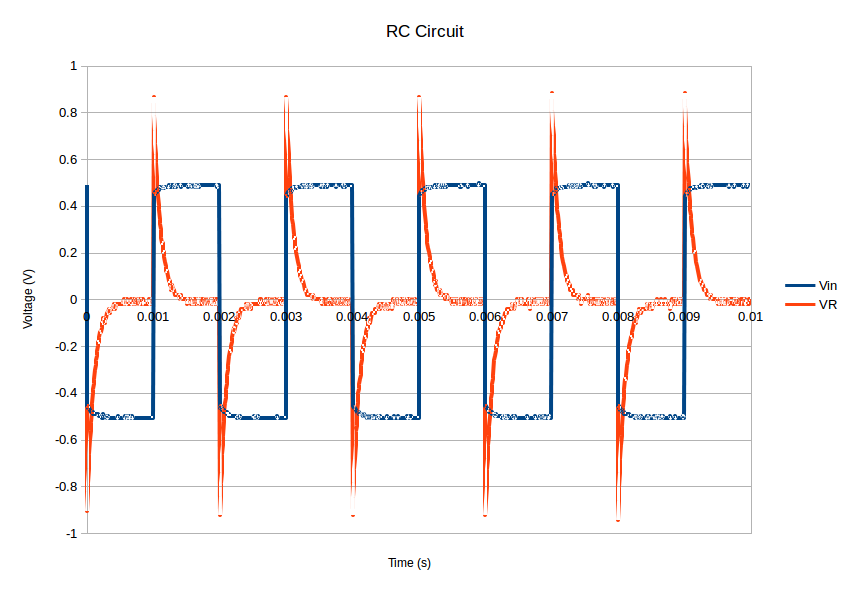
\includegraphics[width=0.7\textwidth]{RC_R.png}
	\caption{Plot of RC circuit measuring $V_R$}
\end{figure}
\begin{figure}[H]
	\centering
	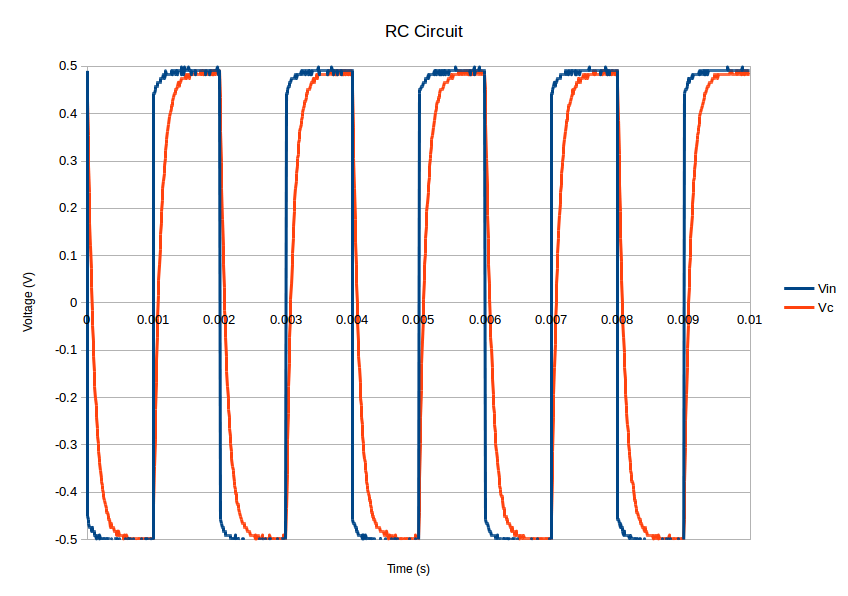
\includegraphics[width=0.7\textwidth]{RC_C.png}
	\caption{Plot of RC circuit measuring $V_c$}
\end{figure}

\subsection*{Nonzero DC Offset}
\begin{figure}[H]
	\centering
	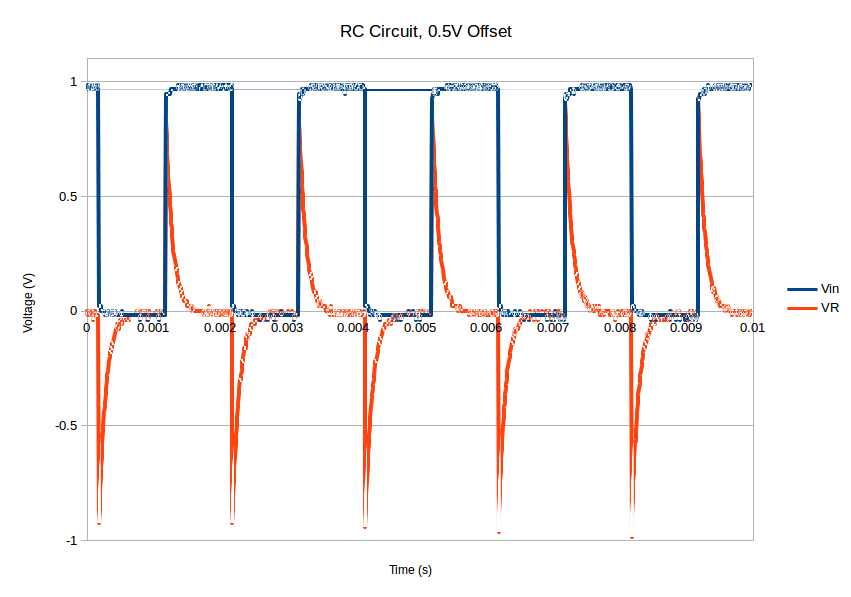
\includegraphics[width=0.7\textwidth]{RC_Offset_R}
	\caption{Plot of RC circuit, 0.5V offset measuring $V_R$}
\end{figure}
\begin{figure}[H]
	\centering
	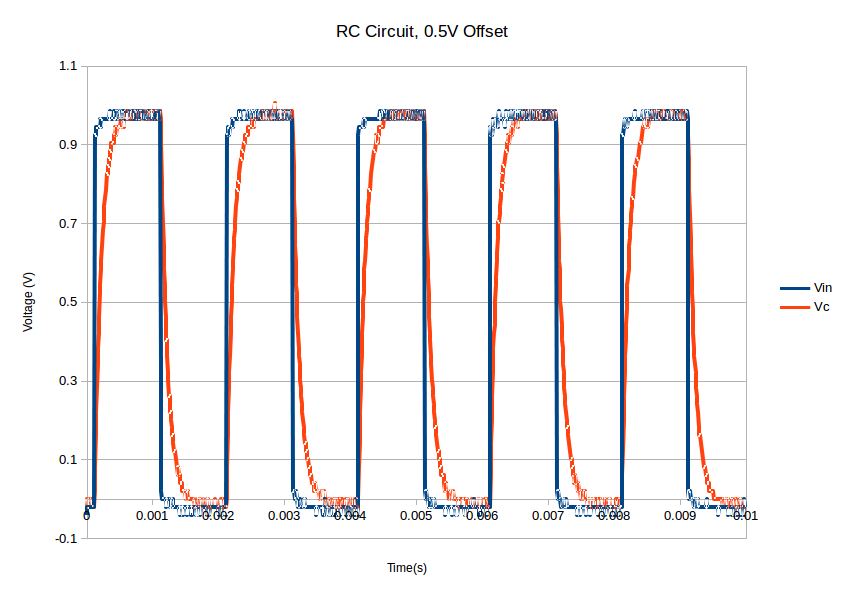
\includegraphics[width=0.7\textwidth]{RC_Offset_C}
	\caption{Plot of RC circuit, 0.5V offset measuring $V_c$}
\end{figure}

\subsection*{Frequency Response}
\begin{figure}[H]
	\centering
	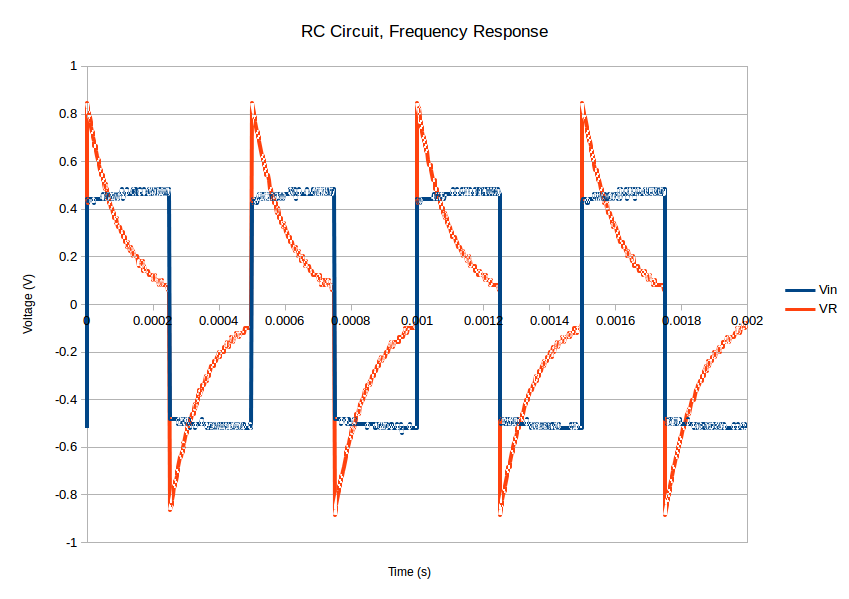
\includegraphics[width=0.7\textwidth]{RC_Frequency_R}
	\caption{Plot of RC circuit, 2kHz measuring $V_R$}
\end{figure}
\begin{figure}[H]
	\centering
	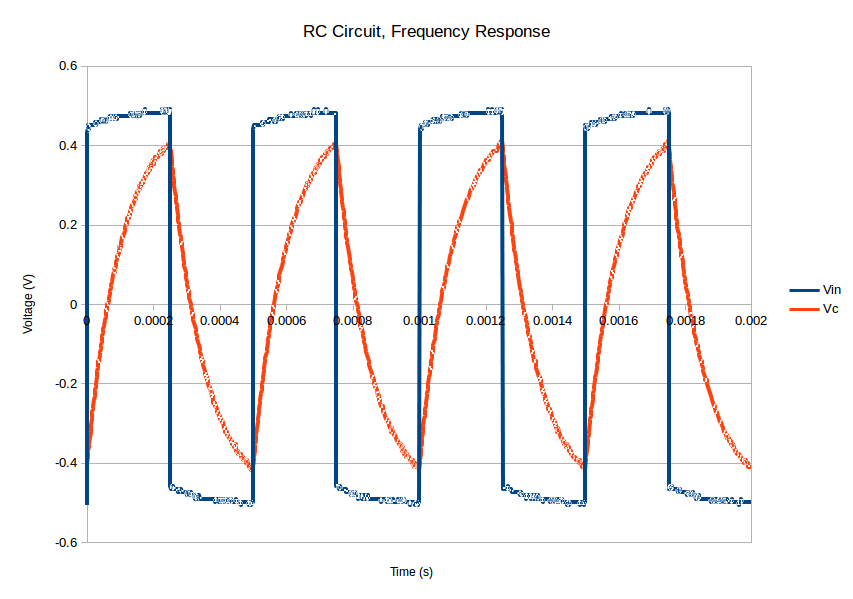
\includegraphics[width=0.7\textwidth]{RC_Frequency_C}
	\caption{Plot of RC circuit, 2kHz measuring $V_c$}
\end{figure}

\subsection*{First Order OP Amp Circuit}
\begin{table}[H]
	\centering
	\begin{tabular}{ll}
		\hline
		\textbf{Element} & \textbf{Measured Value}\\
		\hline
		$R_1$ & $985.92 \Omega$\\
		$R_2$ & $981.50 \Omega$\\
		$R_3$ & $987.64 \Omega$\\
		$C$ & $101.5nF$\\
		\hline
	\end{tabular}
	\caption{Measured values for circuit elements}
\end{table}
\begin{figure}[H]
	\centering
	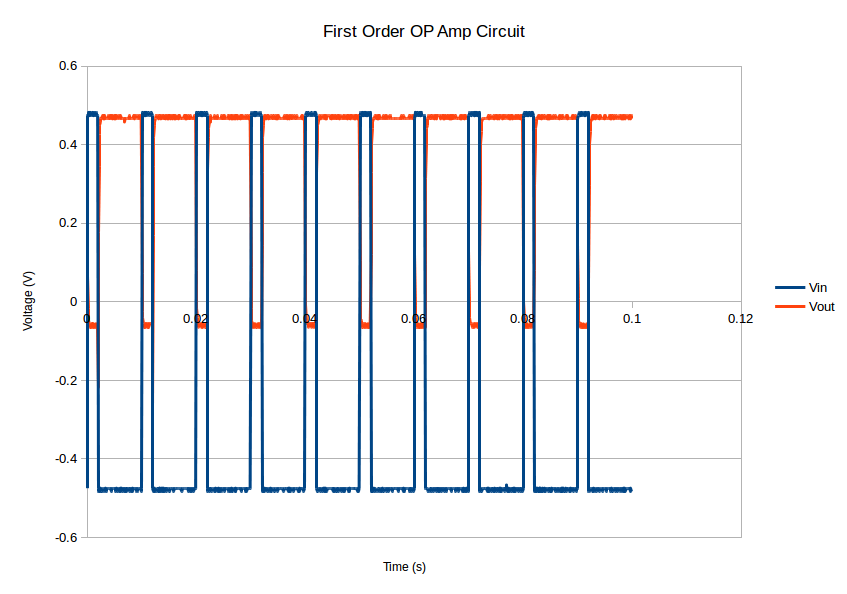
\includegraphics[width=0.7\textwidth]{OPAmp20_100}
	\caption{Plot of first order op amp circuit, 20\% duty cycle, 100Hz}
\end{figure}
\begin{figure}[H]
	\centering
	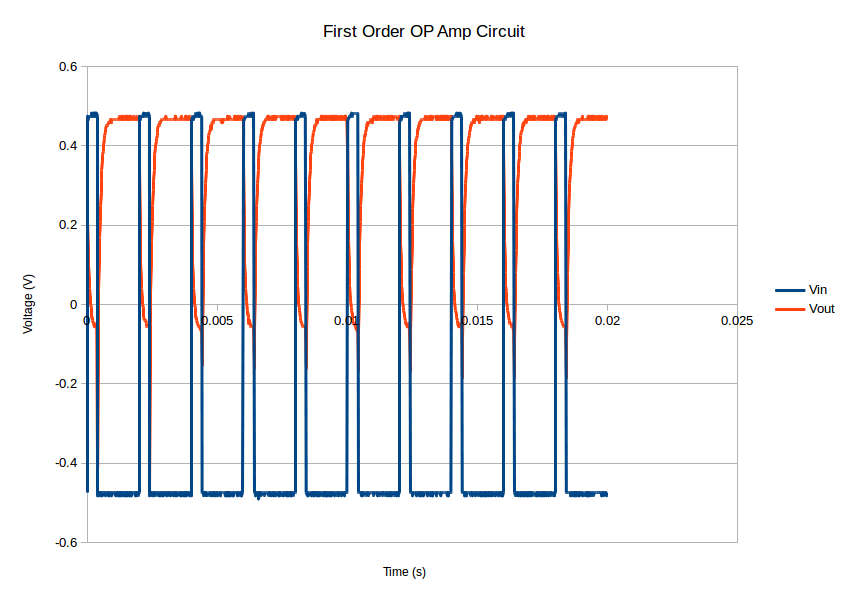
\includegraphics[width=0.7\textwidth]{OPAmp20_500}
	\caption{Plot of first order op amp circuit, 20\% duty cycle, 500Hz}
\end{figure}
\begin{figure}[H]
	\centering
	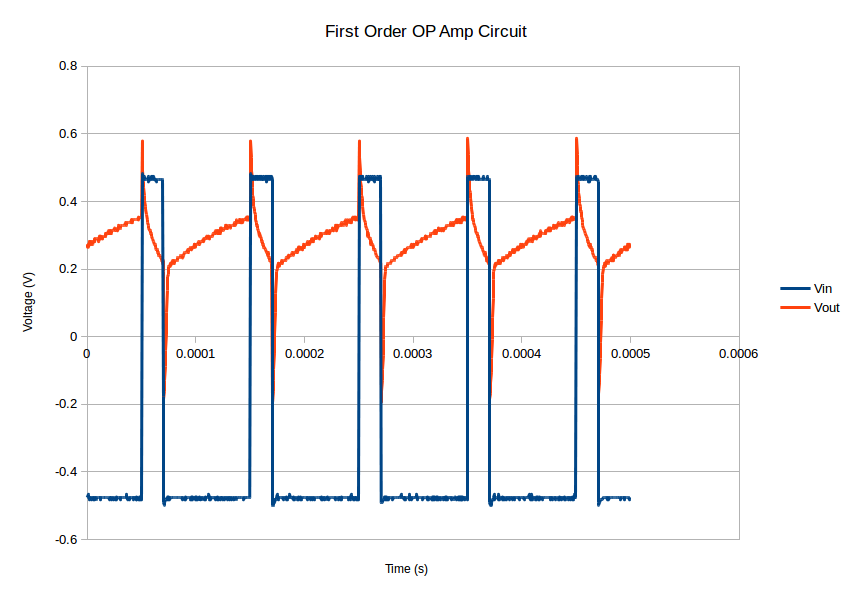
\includegraphics[width=0.7\textwidth]{OPAmp20_10k}
	\caption{Plot of first order op amp circuit, 20\% duty cycle, 10kHz}
\end{figure}
\begin{figure}[H]
	\centering
	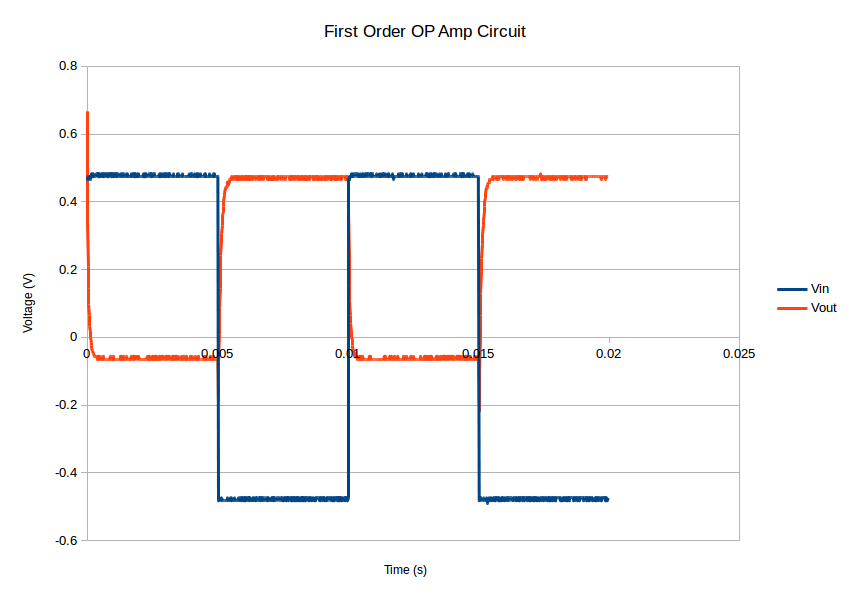
\includegraphics[width=0.7\textwidth]{OPAmp50_100}
	\caption{Plot of first order op amp circuit, 50\% duty cycle, 100Hz}
\end{figure}
\begin{figure}[H]
	\centering
	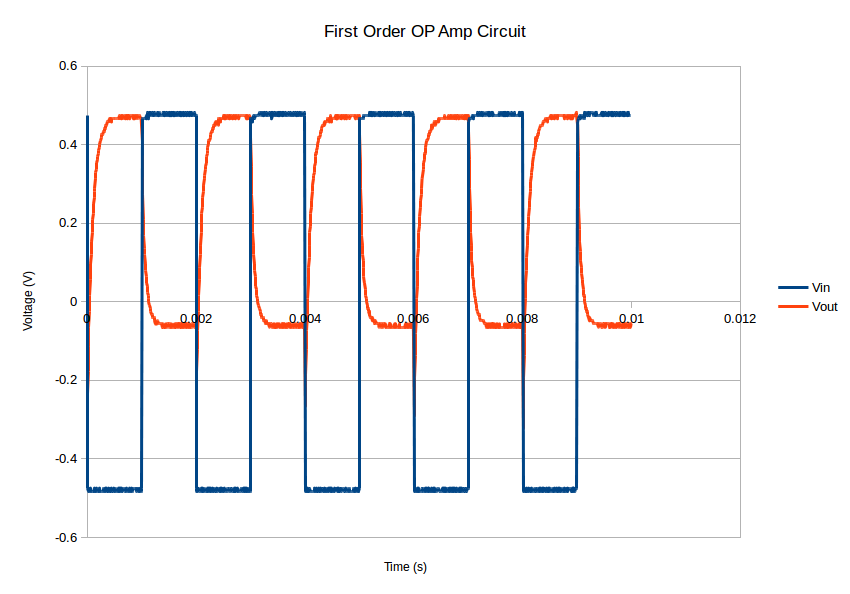
\includegraphics[width=0.7\textwidth]{OPAmp50_500}
	\caption{Plot of first order op amp circuit, 50\% duty cycle, 500Hz}
\end{figure}
\begin{figure}[H]
	\centering
	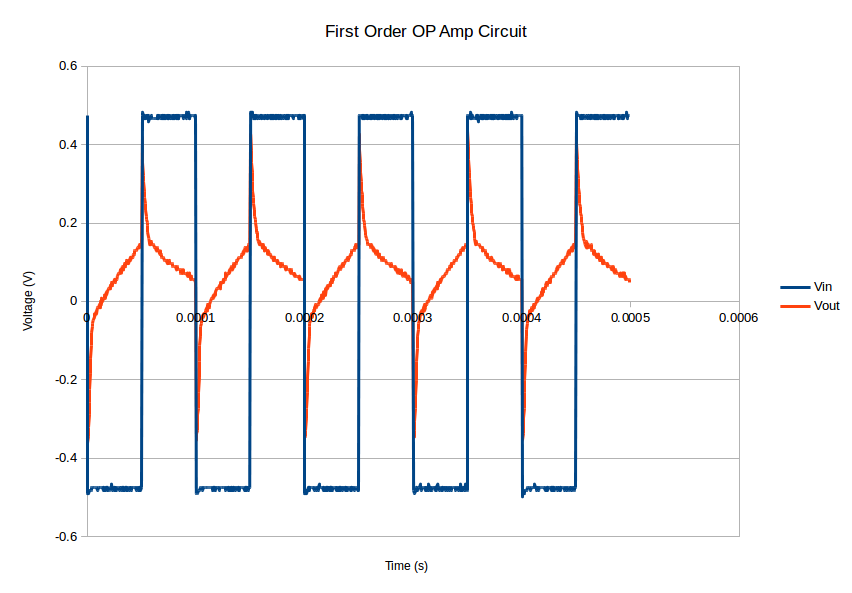
\includegraphics[width=0.7\textwidth]{OPAmp50_10k}
	\caption{Plot of first order op amp circuit, 50\% duty cycle, 10kHz}
\end{figure}

\subsection*{Series RLC Circuit --- Underdamped Response, $R=1k\Omega$}
\begin{table}[H]
	\centering
	\begin{tabular}{ll}
		\hline
		\textbf{Element} & \textbf{Measured Value}\\
		\hline
		Combined Resistance & $990.57 \Omega$\\
		$C$ & $575pF$\\
		$T_1$ & $17\mu s$\\
		$L$ & $10.30mH$\\
		$L_R$ & $23.94\Omega$\\
		\hline
	\end{tabular}
	\caption{Measured values for circuit elements}
\end{table}
\begin{table}[H]
	\centering
	\begin{tabular}{ll}
		\hline
		\textbf{Parameter} & \textbf{Calculated Value}\\
		\hline
		$f_{d,1}$ & $58823.5294 Hz$\\
	\end{tabular}
	\caption{Calculated $f_{d,1}$}
\end{table}
\begin{figure}[H]
	\centering
	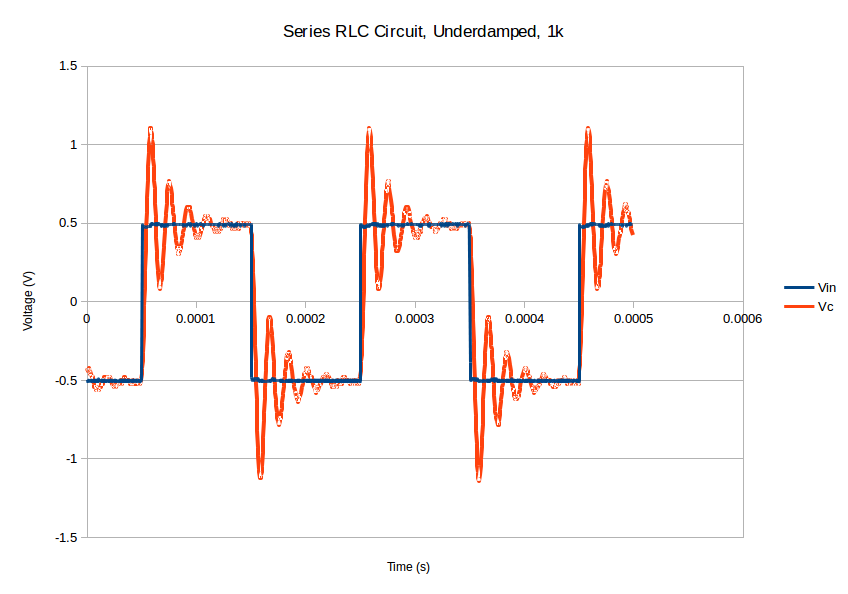
\includegraphics[width=0.7\textwidth]{RLC_Under_1k.png}
	\caption{Plot of Series RLC Circuit --- Underdamped Response, $R=1k\Omega$}
\end{figure}

\subsection*{Series RLC Circuit --- Underdamped Response, Minimum Response}
\begin{table}[H]
	\centering
	\begin{tabular}{ll}
		\hline
		\textbf{Element} & \textbf{Measured Value}\\
		\hline
		Combined Resistance & $1.186 \Omega$\\
		$C$ & $575pF$\\
		$T_1$ & $17\mu s$\\
		$L$ & $10.30mH$\\
		$L_R$ & $23.94\Omega$\\
		\hline
	\end{tabular}
	\caption{Measured values for circuit elements}
\end{table}
\begin{table}[H]
	\centering
	\begin{tabular}{ll}
		\hline
		\textbf{Parameter} & \textbf{Calculated Value}\\
		\hline
		$f_{d,1}$ & $58823.5294 Hz$\\
	\end{tabular}
	\caption{Calculated $f_{d,1}$}
\end{table}
\begin{figure}[H]
	\centering
	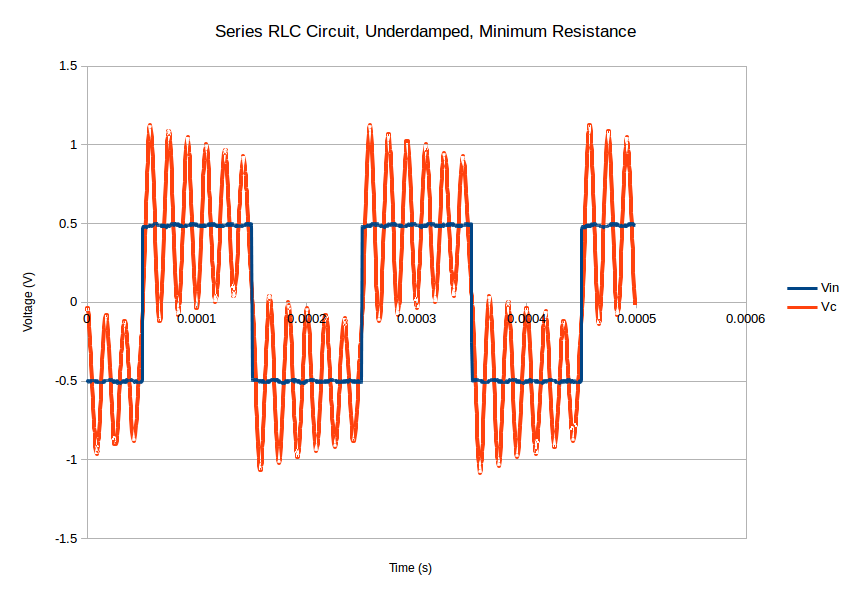
\includegraphics[width=0.7\textwidth]{RLC_Under_Min.png}
	\caption{Plot of Series RLC Circuit --- Underdamped Response, Minimum Response}
\end{figure}

\subsection*{Series RLC Circuit --- Critically Damped Response}
\begin{table}[H]
	\centering
	\begin{tabular}{ll}
		\hline
		\textbf{Element} & \textbf{Measured Value}\\
		\hline
		Combined Resistance & $4.6208 k\Omega$\\
		$C$ & $575pF$\\
		$L$ & $10.30mH$\\
		$L_R$ & $23.94\Omega$\\
		\hline
	\end{tabular}
	\caption{Measured values for circuit elements}
\end{table}
\begin{figure}[H]
	\centering
	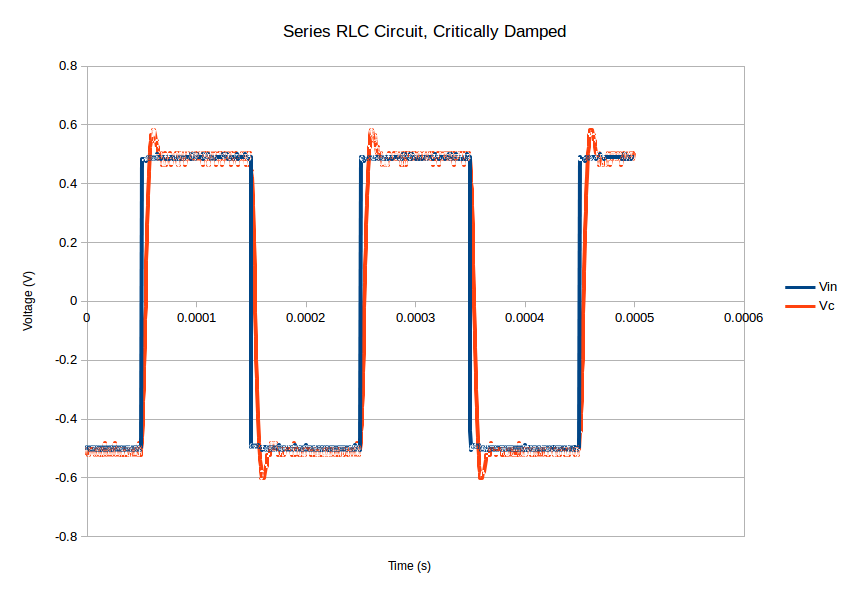
\includegraphics[width=0.7\textwidth]{RLC_Crit.png}
	\caption{Plot of Series RLC Circuit --- Critically Damped Response}
\end{figure}

\subsection*{Series RLC Circuit --- Overdamped Response}
\begin{table}[H]
	\centering
	\begin{tabular}{ll}
		\hline
		\textbf{Element} & \textbf{Measured Value}\\
		\hline
		Combined Resistance & $0.12726 M\Omega$\\
		$C$ & $575pF$\\
		$L$ & $10.30mH$\\
		$L_R$ & $23.94\Omega$\\
		\hline
	\end{tabular}
	\caption{Measured values for circuit elements}
\end{table}
\begin{figure}[H]
	\centering
	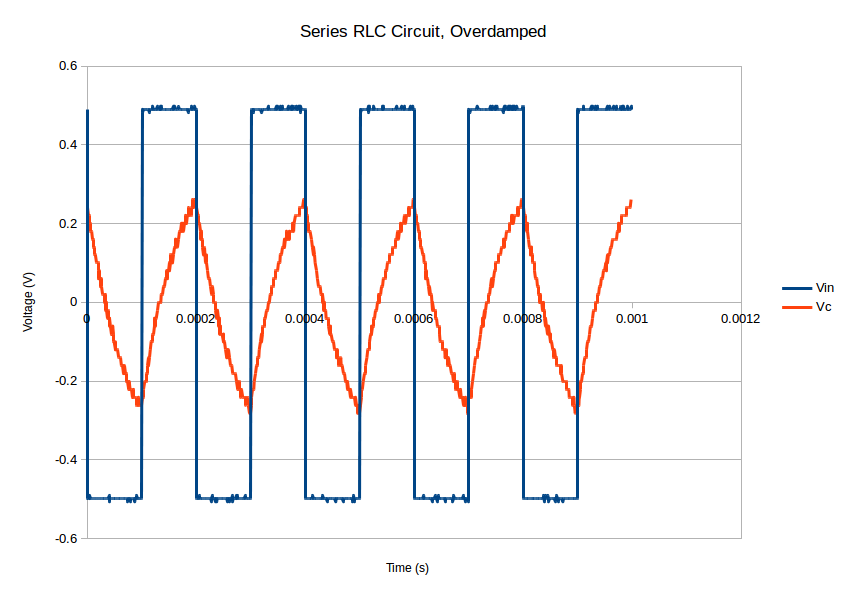
\includegraphics[width=0.7\textwidth]{RLC_Over.png}
	\caption{Plot of Series RLC Circuit --- Overdamped Response}
\end{figure}

\section*{Post-Lab}
\subsection*{Series RC Circuit}
\subsubsection*{Zero DC Offset}
$V_{C,PPK,Calculated} = 0.99995V$\\
$V_{C,PPK,Measured} = 0.99698V$\\
$Percentage Error = \frac{|measured-calculated|}{calculated} = \frac{|0.99698-0.99995|}{0.99995} = 0.297\%$\\
\noindent These values are very close.

\subsubsection*{Nonzero DC Offset}
$V_{C,PPK,Measured,ZeroOffset} = 0.99698V$\\
$V_{C,PPK,Measured,NonZeroOffset} = 1.04523V$\\
$V_{C,PPK,Measured,ZeroOffset} = 1.82915V$\\
$V_{R,PPK,Measured,NonZeroOffset} = 1.90955V$\\
\noindent The waveforms shapes are the same, except the values are shifted by 0.5V.

\subsubsection*{Frequency Response}
$V_{C,PPK,Calculated} = 0.91777$\\
$V_{C,PPK,Measured} = 0.82814$\\
$Percentage Error = \frac{|measured-calculated|}{calculated} = \frac{|0.82814-0.91777|}{0.91777} = 9.766\%$\\
\noindent These values are similar, but differ due to experimental errors.

\subsection*{First Order Op Amp Circuit}
$\tau = RC = (R_1+R_2+R_3)C = (985.92+981.50+987.64)(101.5\times10^{-9} = 2.999\times10^{-4}$
\subsubsection*{100Hz}
\noindent Steady state is reached. 

$T = 5ms$\\
$\frac{5\times10^{-3}}{2.999\times10^{-4}} = 16.67\tau$\\
\noindent The measurements of $v_{out}$ agree with my expectations.

\subsubsection*{500Hz}
\noindent Steady state is reached.

$T = 2ms$\\
$\frac{2\times10^{-3}}{2.999\times10^{-4}} = 6.67\tau$\\
\noindent The measurements of $v_{out}$ agree with my expectations. The larger frequency results in a smaller period, which is reflected in the waveform.

\subsubsection*{10kHz}
\noindent Steady state is not reached.

$T = 50\mu s$\\
$\frac{50\times10^{-6}}{2.999\times10^{-4}} = 0.17\tau$\\
\noindent Due to the high frequency, it was difficult to predict the waveform. However, it was known that the circuit would not reach steady state, which was found to be the case.

\subsection*{Series RLC Circuit}
\subsubsection*{R = 1k$\Omega$}
$f_{calculated,ideal} = 50000 Hz$\\
$f_{calculated,real} = 49705.8252 Hz$\\
$f_{measured} = 58823.5294 Hz$\\
$Percentage Error_{ideal} = \frac{|measured-calculated|}{calculated} = \frac{|58823.5294-50000|}{50000} = 17.65\%$\\
$Percentage Error_{real} = \frac{|measured-calculated|}{calculated} = \frac{|58823.5294-49705.8252|}{49705.8252} = 18.34\%$\\
$T_{calculated,ideal} = 20\mu s$\\
$T_{calculated,real} = 20.1184\mu s$\\
$T_{measured} = 17\mu s$\\
$Percentage Error_{ideal} = \frac{|measured-calculated|}{calculated} = \frac{|17-20|}{20} = 15\%$\\
$Percentage Error_{real} = \frac{|measured-calculated|}{calculated} = \frac{|17-20.1184|}{20.1184} = 15.50\%$\\
\noindent The difference between $\omega_d$ and $\omega_0$ is that $\omega_0$ is the resonant frequency of the circuit, while $\omega_d$ is the imaginary part of the natural frequency of an underdamped circuit.

\subsubsection*{Critically Damped Response}
The experimental data created a waveform that was close to being critically damped, but was not. This is due to the human error in determining when the circuit reaches critical damping, as well as the real values of the circuit elements which are difficult to model.

\subsubsection*{Maximally Damped Response}
\noindent The circuit does reach a new DC steady state during each half period of the square wave.
\end{document}